\documentclass[20pt]{sigchi}


% Use this section to set the ACM copyright statement (e.g. for
% preprints).  Consult the conference website for the camera-ready
% copyright statement.

% Copyright

%\setcopyright{acmcopyright}

%\setcopyright{rightsretained}
%\setcopyright{usgov}
%\setcopyright{usgovmixed}
%\setcopyright{cagov}
%\setcopyright{cagovmixed}
% DOI
% ISBN
%Conference
%Price

% Use this command to override the default ACM copyright statement
% (e.g. for preprints).  Consult the conference website for the
% camera-ready copyright statement.

%% HOW TO OVERRIDE THE DEFAULT COPYRIGHT STRIP --
%% Please note you need to make sure the copy for your specific
%% license is used here!
% \toappear{
% Permission to make digital or hard copies of all or part of this work
% for personal or classroom use is granted without fee provided that
% copies are not made or distributed for profit or commercial advantage
% and that copies bear this notice and the full citation on the first
% page. Copyrights for components of this work owned by others than ACM
% must be honored. Abstracting with credit is permitted. To copy
% otherwise, or republish, to post on servers or to redistribute to
% lists, requires prior specific permission and/or a fee. Request
% permissions from \href{mailto:Permissions@acm.org}{Permissions@acm.org}. \\
% \emph{CHI '16},  May 07--12, 2016, San Jose, CA, USA \\
% ACM xxx-x-xxxx-xxxx-x/xx/xx\ldots \$15.00 \\
% DOI: \url{http://dx.doi.org/xx.xxxx/xxxxxxx.xxxxxxx}
% }

% Arabic page numbers for submission.  Remove this line to eliminate
% page numbers for the camera ready copy
% \pagenumbering{arabic}

% Load basic packages
\usepackage{balance}       % to better equalize the last page
\usepackage{graphics}      % for EPS, load graphicx instead 
\usepackage[T1]{fontenc}   % for umlauts and other diaeresis
\usepackage{txfonts}
\usepackage{mathptmx}
\usepackage[pdflang={en-US},pdftex]{hyperref}
\usepackage{color}
\usepackage{booktabs}
\usepackage{textcomp}
\usepackage{rotating}
\usepackage{listings}
\usepackage{tikz}
\usetikzlibrary{calc}
% Some optional stuff you might like/need.
\usepackage{microtype}        % Improved Tracking and Kerning
% \usepackage[all]{hypcap}    % Fixes bug in hyperref caption linking
\usepackage{ccicons}          % Cite your images correctly!
% \usepackage[utf8]{inputenc} % for a UTF8 editor only

% If you want to use todo notes, marginpars etc. during creation of
% your draft document, you have to enable the "chi_draft" option for
% the document class. To do this, change the very first line to:
% "\documentclass[chi_draft]{sigchi}". You can then place todo notes
% by using the "\todo{...}"  command. Make sure to disable the draft
% option again before submitting your final document.
\usepackage{todonotes}

% Paper metadata (use plain text, for PDF inclusion and later
% re-using, if desired).  Use \emtpyauthor when submitting for review
% so you remain anonymous.
\def\plaintitle{CS524-Project Report}
\def\plainauthor{First Author, Second Author, Third Author,
  Fourth Author, Fifth Author, Sixth Author}
\def\emptyauthor{}
\def\plainkeywords{Authors' choice; of terms; separated; by
  semicolons; include commas, within terms only; required.}
\def\plaingeneralterms{Documentation, Standardization}

% llt: Define a global style for URLs, rather that the default one
\makeatletter
\def\url@leostyle{%
  \@ifundefined{selectfont}{
    \def\UrlFont{\sf}
  }{
    \def\UrlFont{\small\bf\ttfamily}
  }}
\makeatother
\urlstyle{leo}

% To make various LaTeX processors do the right thing with page size.
\def\pprw{8.5in}
\def\pprh{11in}
\special{papersize=\pprw,\pprh}
\setlength{\paperwidth}{\pprw}
\setlength{\paperheight}{\pprh}
\setlength{\pdfpagewidth}{\pprw}
\setlength{\pdfpageheight}{\pprh}

% Make sure hyperref comes last of your loaded packages, to give it a
% fighting chance of not being over-written, since its job is to
% redefine many LaTeX commands.
\definecolor{linkColor}{RGB}{6,125,233}
\hypersetup{%
  pdftitle={\plaintitle},
% Use \plainauthor for final version.
%  pdfauthor={\plainauthor},
  pdfauthor={\emptyauthor},
  pdfkeywords={\plainkeywords},
  pdfdisplaydoctitle=true, % For Accessibility
  bookmarksnumbered,
  pdfstartview={FitH},
  colorlinks,
  citecolor=black,
  filecolor=black,
  linkcolor=black,
  urlcolor=linkColor,
  breaklinks=true,
  hypertexnames=false
}

% create a shortcut to typeset table headings
% \newcommand\tabhead[1]{\small\textbf{#1}}

% End of preamble. Here it comes the document.
\begin{document}
\title{\plaintitle}
\numberofauthors{1}
\author{%
  \alignauthor{Rogers Jeffrey Leo John\\
    \affaddr{University of Wisconsin-Madison}\\
    \affaddr{Madison,WI}\\
    \email{rl@cs.wisc.edu}}\\ 
}

\maketitle
\normal
\section{Introduction}
The problem of scheduling has been extensively studied in the context of a job shop.  Job shop scheduling tries to find an order in which the jobs have to be scheduled on different machines in a plant, taking into account the precedence relationships between jobs and the capacity constraints and tries to minimize the overall time to complete all the jobs. In this paper we examine scheduling in the context of a main memory database system. In particular, we investigate Quickstep, an open source relational database engine designed to efficiently leverage contemporary hardware aspects such as large main memory. 

The work for executing a query in quickstep, can be broken down into of a set of logical units called operators. Each operators is divided into a set of work orders which are the actual units of query execution. We attempt to formulate a model that minimizes the  memory utilization of the Quickstep database system during query execution, by finding an optimal execution order of the work orders. We limit our study to scheduling work orders on a single core.
\vspace{-0.6em}
\section{Background Information} \label{sec:background}
Quickstep is a relational database engine designed to efficiently leverage contemporary hardware aspects such as large main memory, multi-core, and multi-socket server settings.
Query execution in quickstep is controlled by a cost-based query optimizer which produces the query execution plan. Figure~\ref{fig:figure1} shows a SQL query and the corresponding  query plan produced in Quickstep. 

The optimized query plan is  a Directed Acyclic Graph (DAG), where each node in the DAG corresponds to a relational operator primitive (e.g. Build Hash, Probe Hash, Print Output , Drop Output).  Operators can be considered as logical units of work. 
The operators are mapped into  work-orders which are the physical units of work. We present the entire discussion on background information in the context of  operators which can be easily extended to work orders.

Each operator takes some blocks of memory as input. The operators then produce output memory blocks. These output blocks are then consumed by the designated consumer operators in the DAG. 
The whole process repeats until all the operators in the DAG have executed and produced the final result and the final Drop Output operator is executed. 

 An operator can be dependent on multiple operators to complete before it can be scheduled.
The edges in the DAG represent the dependencies between the operators. 
The edge between Probe Hash and Drop hash operators is pipelining because the  Drop Hash operator cannot be scheduled before all the work orders of the Probe Hash operator are complete. 
Similarly, the edge between Probe Hash and Print Output is pipeline breaking or blocking because the work orders of Print Output can be scheduled in parallel with the work orders from Probe Hash. 
At any time T, the operators in the DAG whose dependencies have been meet are considered available for scheduling.
The scheduler schedules work orders from the available operators. The  scheduling of work orders is \textit{non-premptive}
\begin{figure}[ht]

\centering
  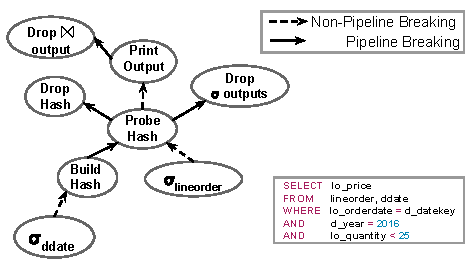
\includegraphics[width=0.9\columnwidth]{figures/QueryPlan}

  \caption{Example of a  query plan produced in Quickstep}~\label{fig:figure1}
  \vspace{-2.0em}
\end{figure}
\vspace{-0.6em}
For a given query, each operator has a \textit{selectivity factor} and a memory requirement associated with it. The selectivity factor is the fraction of input tuples that appear in the output of the operator.The selectivity of an operator can be computed from the data. 
The memory requirement for each operator can be calculated using the formula:  selectivity factor * M, where M is the memory input for a given block. 
The memory requirement of an operator is uniformly distributed across it's work orders.Thus at an any time t, $M_{t}$ units of memory are consumed for query execution. 
The overall memory footprint (MF)  for a query is the sum of  memory units consumed for query execution, over the entire query execution time, i.e. $MF = \sum \limits_{t} M_{t}$
Once an operator completes, the memory consumed by the operator is made available for use by the other operators. 
\vspace{-0.6em}
\section{Problem Statement}
Given a query plan DAG in quickstep, find an optimal ordering of  scheduling work orders, such that the memory footprint is minimized over the entire query execution time. 
\vspace{-0.6em}
\section{Significance}
Identifying the optimal ordering of work orders/operators  for queries is of significance to database researchers, as it helps  in understanding the tradeoffs between query execution times 
and the available memory for query execution. 
\begin{figure}
  \centering
    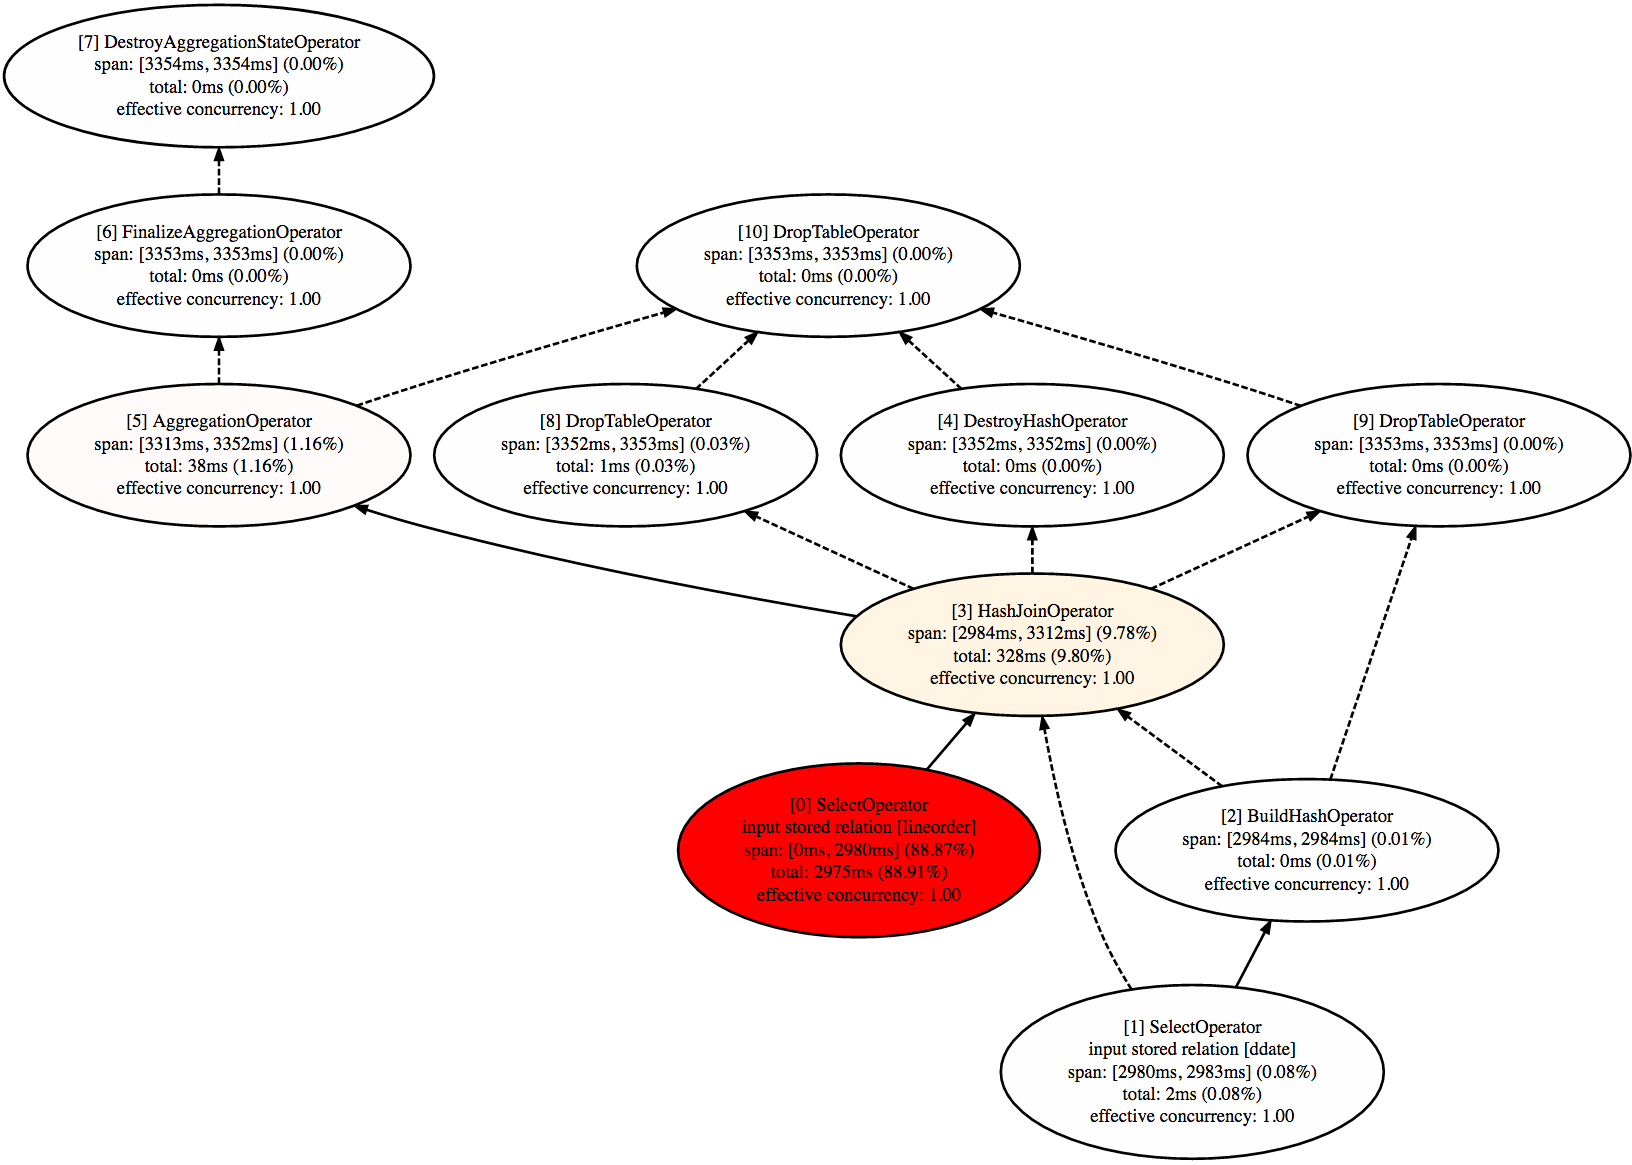
\includegraphics[width=0.5\textwidth]{figures/ssb1}
      \caption{Execution plan for SSB Q-1.1}
      \label{fig2:execution-plan}
\end{figure}
\section{Data Collection}
We collected data regarding the execution times of the different operators, their associated work orders  and their memory requirements by executing queries over a quickstep database instance. Particularly, we collected data for query 1.1 from the Star Schema Benchmark(SSB)~\cite{o2007star}. The execution times of the work orders/operators were measured on a quickstep instance utilizing only a single CPU core. 
% BALANCE COLUMNS
% REFERENCES FORMAT
% References must be the same font size as other body text.
\section{Related Work}
The problem of scheduling has been extensively studied in the context of a job shop. Most of the problem formulations attempt to optimize for time.~\cite{lenstra1978complexity} consider  a machine scheduling problem where the objective function is to minimize the makespan.~\cite{wagner1959integer} describe a rank based model for machine scheduling. 
Similarly, ~\cite{luh1988parallel,hoitomt1990scheduling,luh1990schedule} propose an integer programming formulation to model non-preemptive scheduling of independent jobs for minimizing the weighted tardiness of the job.  Our approach is similar to in that we present  a discrete time integer program formulation  for the problem. However, our objective involves optimizing for memory(resources) as well, instead of just the time.
\section{Model Formulation}
We present a discrete time integer programming formulation to find the optimal ordering of scheduling the work orders in the quickstep database system. We first define the following variables:
\begin {itemize}
\item []\hspace{1em}$o$\hspace{1em}set of all operators
\item[] \hspace{1em}$wo$\hspace{1em}set of all work orders 
\item[] \hspace{1em}$T$\hspace{1em}Total time  for executing the query (Time horizon)
\item[] \hspace{1em}$M$\hspace{1em}represents the mapping between work orders and the  operator
\item[] \hspace{1em}$PRED$\hspace{1em}precedence relationships, indicating that work order i has to complete before work order j
\item[] \hspace{1em}$PIPE$\hspace{1em}pipelining relationships, indicating that work order i has to complete before work order j
\item[] \hspace{1em}$s_{i}$\hspace{1em} start time of the work order i
\item[] \hspace{1em}$e_{i}$\hspace{1em} end time of the work order i
\item[] \hspace{1em}$d_{i}$\hspace{1em} duration of the work order i
\item[] \hspace{1em}$Mem_{i}$\hspace{1em} memory consumed by the work order i
\item []\hspace{1em}$\alpha_{i,k}$\hspace{1em}binary variable equal to one if  work order i was scheduled in time k
\item []\hspace{1em}$\omega_{i,k}$\hspace{1em} binary variable equal to one if work order i ended at time  k
\item []\hspace{1em}$a_{i,k}$\hspace{1em}binary variable equal to one if work order i was active at time k
\item []\hspace{1em}$m_{i,k}$\hspace{1em} binary variable equal to one if  the memory needed by work order i was in use at time k
\end {itemize}
\begin{figure*}[t]
  \centering
    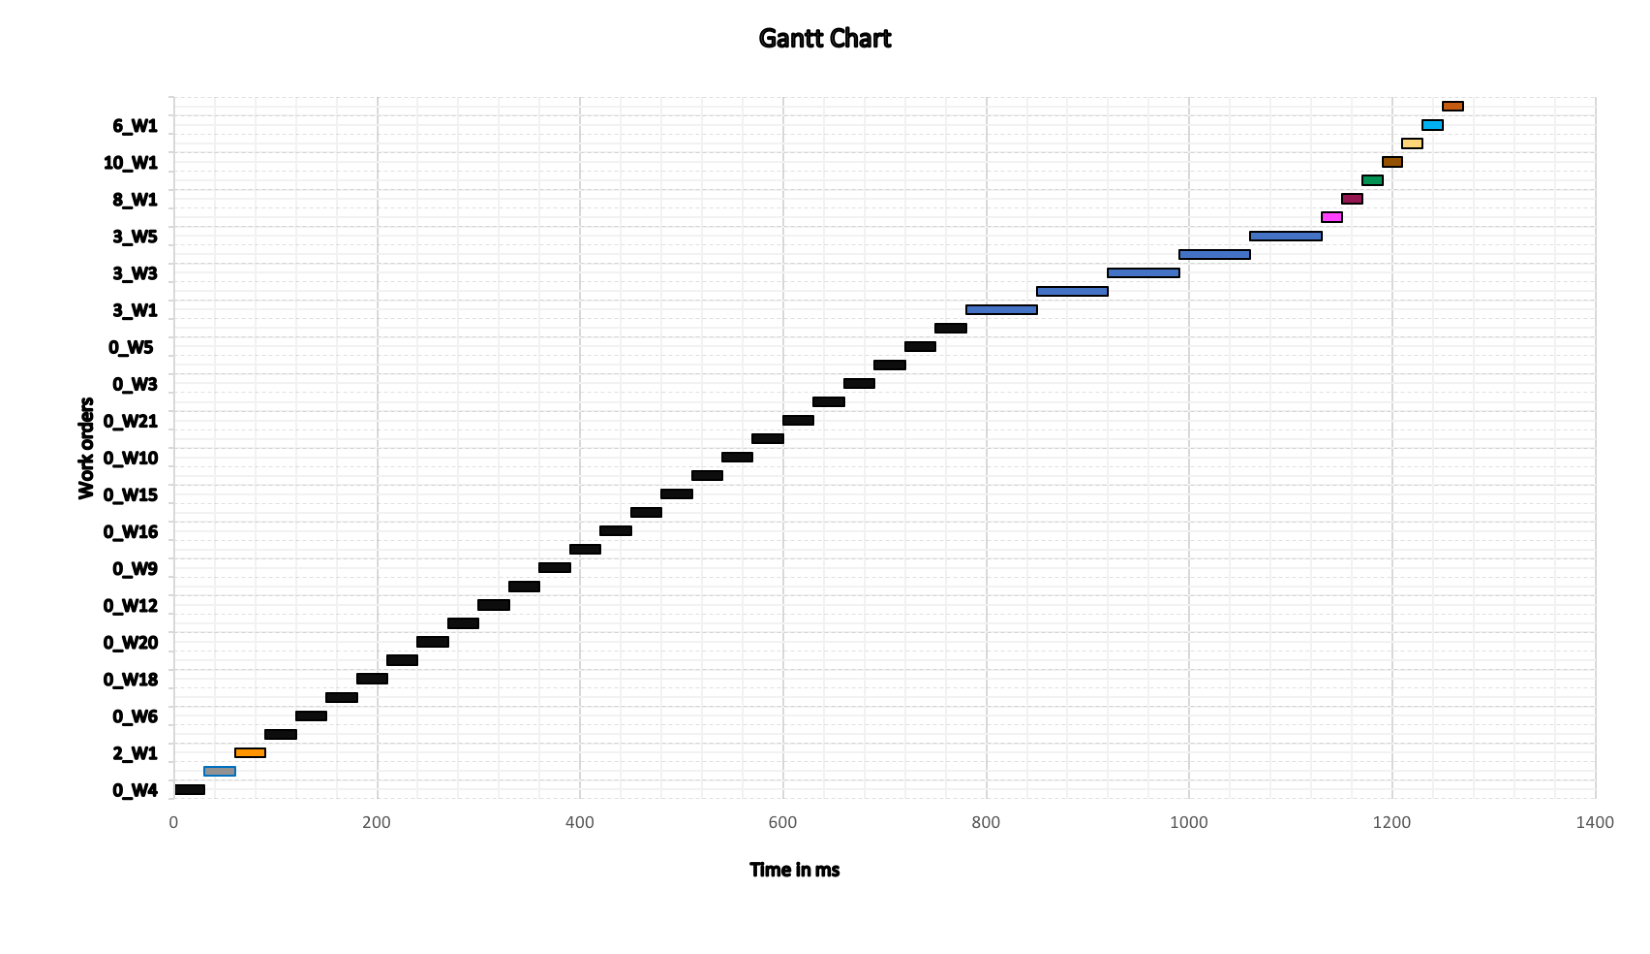
\includegraphics[width=0.95\textwidth]{figures/GanttChart}
   	\label{fig3:gantt-chart}
	      \caption{Gantt chart showing the execution order if the operators. Duration of each work order has been rounded off to the nearest milli second}
\end{figure*}
We assume that the the work orders are being scheduled on a single core, i.e only one work order can be scheduled at a time.
This is expressed by the equation:
\begin{equation}
%sum(I,wo_scheduled(t,I)) =l= 1;
\sum\limits_{i \in wo} \alpha_{i,k} =1\hspace{1em}\forall k = 1 \hdots  T
\end{equation}
A work order  has to be active over the entire duration of its execution. Therefore, the following equation holds by definition:
\begin{equation}
%wo_active(T,I) =e= wo_active(T-1,I)+wo_scheduled(t,I)-wo_ended(t,I);
     a_{i,k} =a_{i,k-1} + \alpha_{i,k}-\omega_{i,k}\hspace{1em}   \forall i \in wo, k = 1 \hdots  T
\end{equation}
Further, since this is a single core system, new work orders cannot be scheduled/processed as  long as the core is busy with an existing work order.  The following equation expresses this. 
\begin{equation}
%sum(I,wo_active(t,I)) =l=1;
\sum\limits_{i \in wo} a_{i,k} =1\hspace{1em}\forall k = 0 \hdots  T
\end{equation}
A job, once completed cannot be scheduled again. This constraint is expressed by the following equation.
\begin{equation}
%sum(t,wo_scheduled(t,I)) =e= 1;
\sum\limits_{k=1}^{T} \alpha_{w,k}  =1\hspace{1em}\forall w \in wo
\end{equation}
As described in the background information, precedence relationships exist among operators and these precedence relationships can be blocking or non-blocking(pipelining). 
If  an operator B is blocking on operator A, then all the work orders of operator A should be scheduled before the work orders of operator B.
We express the blocking  precedence relationships between the operators through the following constraint:
\begin{equation}
\label{eqn:5}
%start(J) =g= start(I) + duration(I);
s_{w_{B}} > s_{w_{A}} + d_{w_{A}}\hspace{1em} \forall (w_{A},w_{B}) \in PRED
\end{equation} 
We also describe a second type of precedence called pipelining, wherein two operators A,B who are pipelined  can have their work orders scheduled in an interleaved fashion.
Let us consider two operators A and B whose work orders are  $w_{A1}$, $w_{A2}$, $w_{A3}$ and $w_{B1}$, $w_{B2}$ 
respectively.  A valid schedule could be  $w_{A1}$, $w_{B1}$, $w_{A2}$, $w_{A3}$ , $w_{B2}$. 
The following  equation expresses this pipelining relationship:
\begin{multline}
\label{eqn:6}
%sum ((I,T)$(map(O1,I) and ord(T)<=ord(T1)),wo_ended(T,I)) =g= sum ((J,T)$(map(O2,J) and %ord(T)<=ord(T1)),wo_scheduled(T,J));
\sum\limits_{i,k}\omega_{i,k} \mid i,A \in M , k <=T_{t}
\\<= \sum\limits_{i,k}\omega_{j,k} \mid j,B \in M, k <=T_{t}  \\ \forall (A,B) \in PIPE  \hspace{1em} , T_{k}= 1 \hdots T \hspace{1em}
A \in o, B \in o
\end{multline}
The equation enforces that  if operator A is pipelined to B, then the number of work orders  of operator A that are complete should be greater than or equal to the number of work orders completed to operator B.
However, this does not eliminate invalid  schedules like $w_{A1}$, $w_{B1}$, $w_{B2}$, $w_{A2}$ , $w_{A3}$, where there are no outputs produced to consume the data produced by  work orders $w_{A2}$  and $w_{A3}$. To avoid this we introduce a new constraint,
\begin{equation}
\label{eqn:7}
%sum ((I,T)$(map(O1,I)),ord(T)*wo_ended(T,I)) =l= sum ((J,T)$(map(O2,J)),ord(T)*wo_ended(T,J));
\sum\limits_{i,k} k  * \omega_{i,k}  \mid i,A \in M ,
<=
\sum\limits_{j,k} k  * \omega_{j,k}  \mid j,b \in M ,  k = 1 \hdots T
\end{equation} 

This constraint enforces that, the end time of the operator B (which is at the end of the pipeline), should be greater than  the end time of the operator A(which is at the beginning of the pipeline). 

Finally, we describe our objective equation. The objective equation consist of  two parts.
\begin{equation}
\label{eqn:8}
%memory_footprint =e= sum(I,memory_consumption(I)*(total_task_duration-start(I)))+ sum(I,start(I))
\sum \limits_{i \in wo} Mem_{i} * (T - s_{i}) +  \lambda \sum  \limits_{i \in wo} s_{i}
\end{equation} 
The first part of the objective equation calculates the total memory occupied by every work order during the query equation.
Recall that, though a work order completes it's memory is not released until a DropTable work order is invoked. Thus the memory stays active until it is destroyed. But our model does not have a notion of destroy work orders built into it. We handle such destroy work orders by specifying in the data that work orders belonging to an operator of type destroy have negative memory.

Therefore, to calculate the memory consumption,  we assume that the work order occupies memory through the entire duration query execution. Thus, for  the work orders  who have positive memory requirements and negative memory requirements , they end up occupying memory right from the instant they were scheduled until the entire query execution completes. The net effect of this formulation is that, a work order's memory is counted  until the time a corresponding destroy work order gets scheduled.

The second part of the of the objective equation minimizes the total  start time over all the work orders. The parameter lambda  can be used to control the tradeoff between minimizing for time and memory.
\section{Results}
We present our results of the model for Query 1.1 of the SSB Benchmark: 
\begin{lstlisting}[language=sql,basicstyle=\ttfamily,breaklines=true,morekeywords={*,select},]
select sum(lo_extendedprice*lo_discount) as revenue
from lineorder, ddate
where lo_orderdate = d_datekey
		and d_year = 1993
		and lo_discount between 1 and 3
		and lo_quantity < 25;
\end{lstlisting}
The query involves a  join between the fact table lineorder and the dimension table ddate followed by an aggregation on the product of the discount and the price attributes of the lineorder table. The query also  involves filtering of  the ddate table  based in the d\_year attribute and the lineorder table based  on the lo\_discount and lo\_quantity attributes.
Figure ~\ref{fig2:execution-plan} shows the execution DAG for  Query 1.1.  There are 10 operators in the DAG corresponding to the selection filtering , aggregation operations. There are also destroy operators free the memory occupied by the various operators over the query execution. The arrows between the operators indicate the precedence relationships between the operators.

Figure~\ref{fig3:gantt-chart} presents the ordering of the work orders  obtained as an output during the solve of the model. 
It can be seen that work orders from $0$, $1$  and $2$ as interleaved as they do not have precedence relationships.
However, since $1$  and $2$  have a pipelining relationship associated with them (as seen from  Figure 2), they are scheduled in sequence. Also, since $3$ is blocked on $1$, all work orders of $3$ are scheduled only after all work orders of $1$ are scheduled.

Similarly the schedule respects the precedence for the other operators.  Work orders of  operators $4$, $9$  and $2$ which are \textit{DropTable} operators , are scheduled immediately after work orders of $3$ are scheduled.  These operators correspond to releasing the memory used by operators $0$, $1$  and $3$ respectively. Although, operators $5$ and $6$  are available for scheduling, the schedule gives priorities to the destroy operators that free memory, there by reducing the amount of memory that is in use. We can therefore see that the scheduler presented by the model optimizes for the memory usage.

Figure~\ref{fig4:memory-consumption} shows the memory consumed by the work orders during query execution. The figure has been simplified to show the memory in use only when a work order is scheduled. The drop in memory corresponds to the DropTable work orders being scheduled.

\begin{figure}
  \centering
    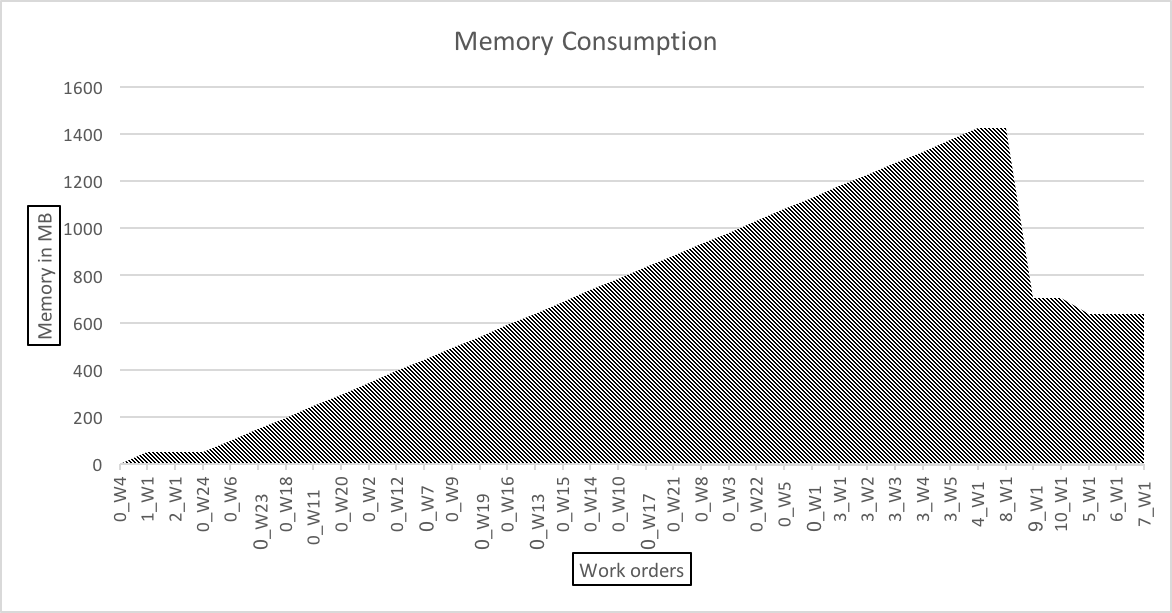
\includegraphics[width=0.5\textwidth]{figures/memory_utilization}
      \caption{Memory Consumption over the query execution time.}
      \label{fig4:memory-consumption}
\end{figure}
\section{Limitations}
Representing time as a discrete unit has a limitation of causing the model to blow up for really huge data sets. This is mainly because increasing the size of the data, increases the number of work orders produced thereby increasing the overall processing time of the query. 
\section{Future Work}
An important aspect of this work, is to extend the model to multi-core settings. The current design of the model lends itself to be easily extended to a multi core setting.   We would also like to address the limitations of the current model by extending and tuning it to scale for query execution on several Gigabytes of data. It would also be interesting to compare the results with the current execution ordering in the Quickstep main memory database system.
\bibliographystyle{SIGCHI-Reference-Format}
\bibliography{sample}

\end{document}

%%% Local Variables:
%%% mode: latex
%%% TeX-master: t
%%% End:
